
\section{LaneRCNN}


Our goal is to  predict the future motions of all actors in a scene, given their
past motions and an HD map. Different from existing work, we represent an actor
and its context with a \textit{LaneRoI}, an actor-specific graph representation which is more
structured and expressive than the single feature vector used in the literature. 
Based
on this representation, we design LaneRCNN, a graph-centric motion forecasting
model that encodes context, models interactions between actors, and predicts future motions all in
a map topology aware manner. An overview of our model is shown in
Fig.~\ref{fig:lanercnn}.

In the following, we first introduce our problem formulation 
in Sec. \ref{sec:notation}. We then define our \ROI representations in Sec.
\ref{sec:laneroi}. In Sec. \ref{sec:backbone}, we explain how LaneRCNN processes features and models interactions via graph-based message-passing. 
Finally, we show our map-aware trajectory decoder and learning
in Sec. \ref{sec:output} and Sec. \ref{sec:learning} respectively.






\subsection{Problem Formulation}
\label{sec:notation}
We denote the  past motion of the $i$-th actor as a set of 2D points encoding
the center locations over the past $L$ 
 timesteps, \ie, $\left\{(x_i^{-L}, y_i^{-L}), \cdots, (x_i^{-1},
y_i^{-1})\right\}$, with $(x,y)$  the  2D coordinates  in bird's eye view (BEV). Our goal is to forecast the future motions of all actors in the scene 
$\left\{(x_i^{1}, y_i^{1}), \cdots, (x_i^{T}, y_i^{T}) | i = 1, \cdots, N\right\}$,
where $T$ is our prediction horizon and $N$ is the number of actors. 

In addition to the past kinematic information of the actors, maps also play an important role 
for motion forecasting since (i) actors usually follow lanes on the map, 
(ii) the map structure determines the right of way, which in turns affects the interactions among actors.
As is common practice in self-driving, we assume an HD map is accessible, 
which contains lanes and associated semantic attributes, \eg,
traffic light information. 
Each lane is composed of
many consecutive lane segments $\ell_i$, which are short segments
along the centerline of the lane.
In addition, a lane segment $\ell_i$ can have pairwise relationships with
another segment $\ell_j$ in the same or another lane, 
such as $\ell_i$ being a successor of $\ell_j$ or a left neighbor.

\subsection{LaneRoI Representation}
\label{sec:laneroi}


\paragraph{Graph Representation}
One straight-forward way to represent an actor and its context (map) information
is by first rasterizing both its trajectory as well as the map to form a 2D BEV
image, and then apply cropping centered in the actor's location in BEV \cite{dsd, mfp, matf, spagnn}.
However, rasterizations are prone to information loss such as 
connectivities among lanes. 
Furthermore, it is a rather inefficient representation
since actor motions are expanded typically in the direction along the lanes, not across them. 
Inspired by \cite{lgn}, we instead use a graph representation for our \ROI to
preserve the structure while being compact. For each actor $i$ in the scene, we first
retrieve all relevant lanes that this actor can possibly go to in the prediction horizon
$T$ as well as come from in the observed history horizon $L$. We then convert the
lanes into a directed graph $\G_i =
\{\mathcal{V}, \{ \mathcal{E}_\text{suc}, \mathcal{E}_\text{pre},
    \mathcal{E}_\text{left}, \mathcal{E}_\text{right} \}\}$
where each node $v \in \mathcal{V}$ represents a lane segment within those lanes 
and the lane topology is represented by different types of edges $\mathcal{E}_r$,
encoding the following relationships: predecessor, successor, left
and right neighbor.  
Two nodes are connected by an edge $e \in \mathcal{E}_r$ if the corresponding lane segments $\ell_i,
\ell_j$ have a relation $r$, \eg, lane segment $\ell_i$ is a
successor of lane segment $\ell_j$.
Hereafter, we will use the term node interchangeably with the term lane segment. 











\paragraph{Graph Input Encoding}
The graph $\G_i$ only characterizes map structures around the $i$-th actor without much information about the actor.
We therefore augment the graph with a set of node embeddings to
construct our \textit{LaneRoI}.
Recall that each node $k$ in $\G_i$ is associated with a lane
segment $\ell_k$. We design its embedding $f_k \in \mathbb{R}^C$ 
to capture the geometric and semantic information of
$\ell_k$, as well as its relations with the actor, where $C$ denotes the feature
dimension.
In particular, geometric features include the center location, the orientation and the
curvature of $\ell_k$; semantic features include binary features indicating if
$\ell_k$ is a turning lane,  if it is currently controlled by a red light,
\etc. To encode the actor information into $f_k$, we note that the past motion of an
actor can be identified as a set of 2D displacements, defining the 
movements between consecutive timesteps. Therefore, we also include the relative
positions and orientations of these 2D displacements \wrt $\ell_k$
into $f_k$ which encodes actor motions in a map-dependent manner.
This is beneficial for understanding actor behaviors \wrt the map, \eg, a trajectory that 
steadily deviates from one lane and approaches the neighboring lane is highly likely 
a lane change.
In practice, it is important to clamp the actor information, \ie, if $\ell_k$ is more than 5 meters away from the
actor we replace the actor motion embedding in $f_k$ with zeros. 
We hypothesize that such a restriction encourages the model to learn better representations via the message passing over the graph.
To summarize, $(\G_i, \mathbf{F}_i)$ is the \ROI of the actor $i$, encoding
the actor-specific information for motion forecasting,
where $\mathbf{F}_i \in
\mathbb{R}^{M_i \times C}$ is the collection of node embeddings $f_k$ and 
$M_i$ is the number of nodes in $\G_i$. 

\begin{figure}[t]
\begin{center}
  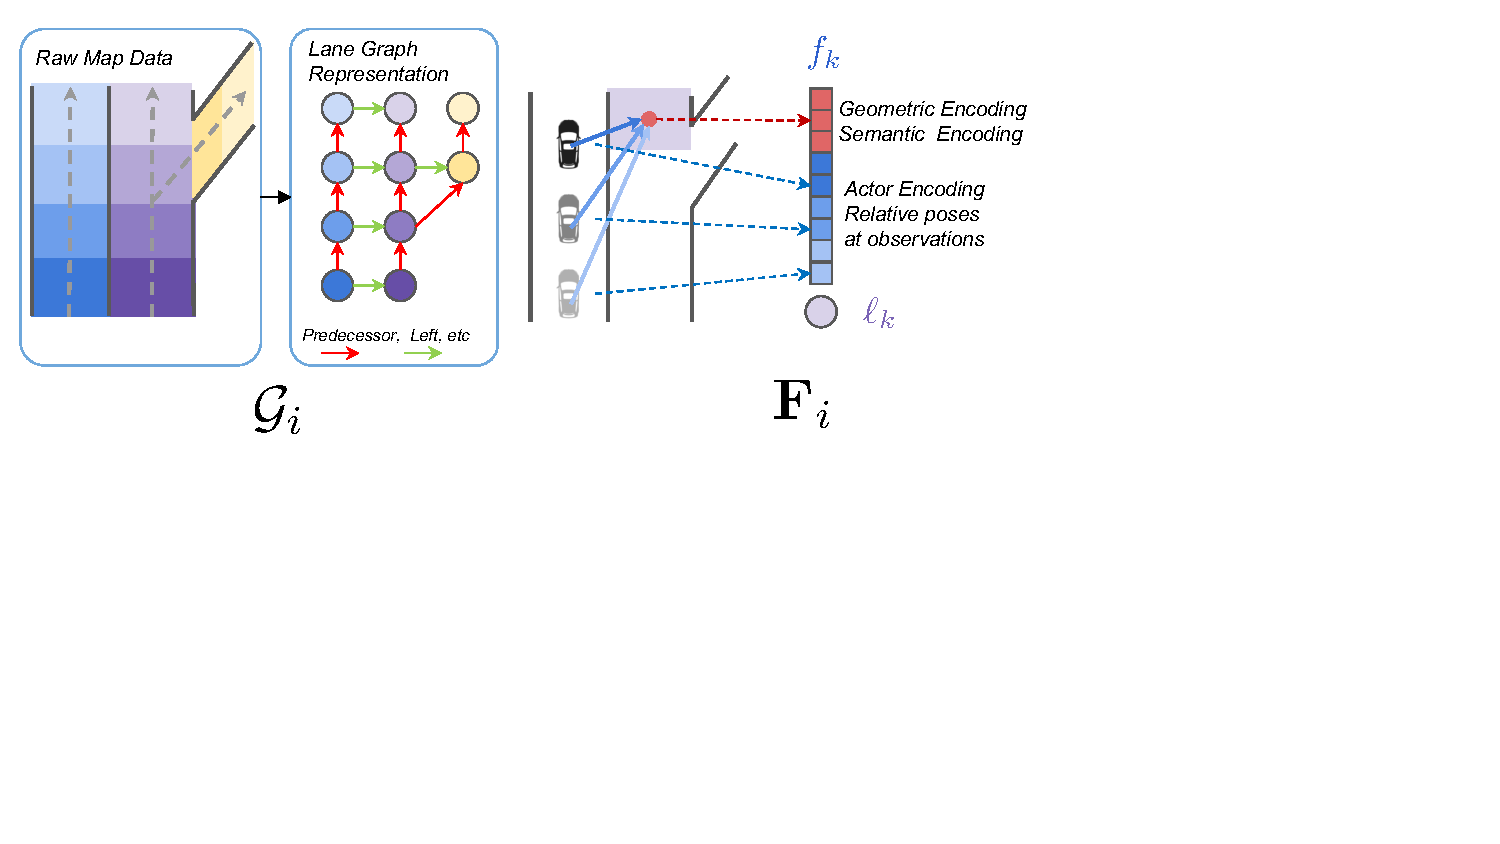
\includegraphics[height=3.4cm]{figures/laneroi.pdf}
\end{center}
\vspace{-0.2cm}
\caption{
The LaneRoI of the actor $i$ is a collection of a graph $\G_i$ (constructed following lane topology: nodes as
lane segments and edges as segment connectivities) and node
embeddings $\mathbf{F}_i$ (encoding motions of the actor, as well as
geometric and semantic properties of lane segments).}
\vspace{-0.3cm}
\label{fig:laneroi}
\end{figure}


\subsection{LaneRCNN Backbone}
\label{sec:backbone}
As \textit{LaneRoI}s have irregular graph structures, we can not apply standard
2D convolutions to obtain feature representations. In the following, we first introduce
the lane convolution and pooling operators (Fig.~\ref{fig:operator}), which serve similar
purposes as their 2D counterparts while respecting the graph topology. 
Based on these operators, we then describe how our LaneRCNN updates features of
each \ROI as well as handles interactions among all \textit{LaneRoI}s (actors).


\paragraph{Lane Convolution Operator}
We briefly introduce the lane convolution which was originally proposed in \cite{lgn}
Given a \ROI $(\G_i, \mathbf{F}_i)$, 
a lane convolution updates features $\mathbf{F}_i$ by aggregating features from
its neighborhood (in the graph). 
Formally, we use $\E_i(r)$ to denote the 
binary adjacency matrix for $\G_i$ under the relation $r$, \ie, the $(p, q)$ entry 
in this matrix is $1$ if lane segments $\ell_p$ and $\ell_q$ have the relation $r$ 
and $0$ otherwise. 
We denote the $n$-hop connectivity under the relation $r$ as the matrix 
$\bool\left(\E_i(r) \cdot \E_i(r) \cdots \E_i(r)\right) = \bool
\left(\E_i^n(r)\right)$, where the operator $\bool$ sets any non-zero entries to one 
and otherwise keeps them as zero. 
The output node features are updated as follows,
\begin{equation}
  \label{eq:conv}
  \mathbf{F}_i \leftarrow \Psi \left( \mathbf{F}_i\mathbf{W} + \sum_{r, n}
  \bool \left(\E_i^n(r)\right)\mathbf{F}_i\mathbf{W}_{n, r} \right),
\end{equation}
where both $\mathbf{W}$ and $\mathbf{W}_{n, r}$ are learnable
parameters, $\Psi(\cdot)$ is a non-linearity consisted of
LayerNorm \cite{layernorm} and ReLU \cite{relu},
and the summation is over all possible relations $r$
and hops $n$. In practice, we use 
$n \in \left\{1, 2, 4,
8, 16, 32\right\}$.
Such a multi-hop mechanism mimics the dilated convolution \cite{yu2015multi} and effectively enlarges
the receptive field.

\begin{figure}[t]
\begin{center}
  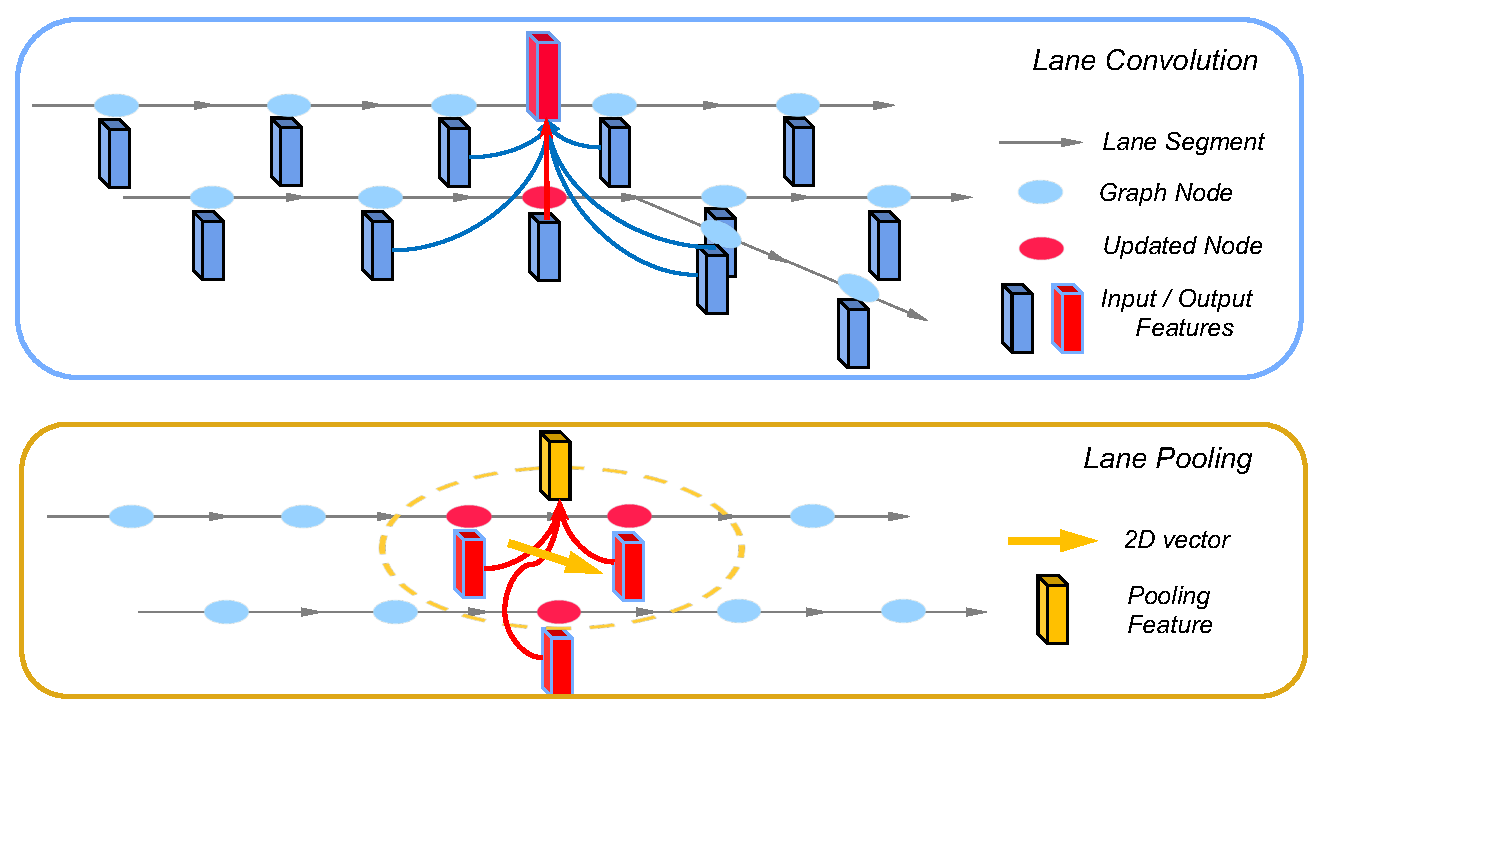
\includegraphics[height=4.5cm]{figures/operator.pdf}
\end{center}
\vspace{-0.2cm}
\caption{An illustration for lane convolution and lane
pooling operators, which have similar functionalities as their 2D counterparts
while respecting the lane topology.}
\label{fig:operator}
\end{figure}


\paragraph{Lane Pooling Operator}
We use a learnable pooling function for lane pooling operator.
Given a \ROI
$(\G_i, \mathbf{F}_i)$, recall $\G_i$ actually corresponds to a number of
lanes spanned in the 2D plane (scene). For an arbitrary 2D vector
$\mathbf{v}$ in the plane, a lane pooling operator pools, or `interpolates',
the feature of $\mathbf{v}$ from $\mathbf{F}_i$. Note that
$\mathbf{v}$ can be a lane segment in another graph $\G_j$ (spatially
close to $\G_i$). Therefore, lane pooling helps
communicate information back and forth between graphs, which we will explain in the interaction part.
To generate the feature $f_\mathbf{v}$ of vector $\mathbf{v}$, we first retrieve
its `neighboring nodes' in $\G_i$, by checking if the center distance between a lane segment
$\ell_k$ in $\G_i$ and vector $\mathbf{v}$ is smaller than a certain threshold. A naive
pooling strategy is to simply take a mean of those $\ell_k$. However, this
ignores the fact that relations between $\ell_k$ and $\mathbf{v}$ can vary a lot
depending on their relative pose: a lane segment that is perpendicular to
$\mathbf{v}$ (conflicting) and the one that is aligned with $\mathbf{v}$
have very different semantics. Inspired by the generalized convolution on graphs/manifolds
\cite{monti2017geometric, contconv, lgn}, we use the relative pose and some non-linearities to
learn a pooling function. In particular, we denote the set of surrounding
nodes on $\G_i$ as $\mathcal{N}$, and the relative pose between $\mathbf{v}$ and
$\ell_k$ as $\Delta_{\mathbf{v}k}$ which includes relative position and
orientation. The pooled feature $f_{\mathbf{v}}$ can then be written as,
\begin{equation}
  \label{eq:pool}
  f_{\mathbf{v}} = \mathcal{M}_b\left(\sum_{k\in \mathcal{N}}
    \mathcal{M}_a\left(\left[
        f_k, \Delta_{\mathbf{v}k}
\right]\right)\right),
\end{equation}
where $[\cdots]$ means concatenation and $\mathcal{M}$
is a two-layer multi-layer perceptron (MLP).



\begin{table*}[t]
\vspace{-0.2cm}
\centering
\begin{tabular}{l|>{\columncolor{grey}}cccccc}
  \specialrule{.2em}{.1em}{.1em}
  Method & MR (K=6) & minADE (K=6) & minFDE (K=6) & MR (K=1) & minADE (K=1) & minFDE (K=1) \\
  \hline
   NN+Map~\cite{argoverse} & 58.0 & 2.08 & 4.02 & 94.0 & 3.65 & 8.12\\
   LSTM+Map~\cite{argoverse} & 67.0 & 2.08 & 4.19 & 75.0 & 2.92 & 6.45\\
   UULM-MRM~\cite{argoleaderboard} & 21.8 & 0.97 & 1.55 & 63.4 & 1.90 & 4.19\\
   WIMP~\cite{wimp} & 16.7 & 0.99 & 1.67 & 62.9 & 1.82 & 4.03\\ 
   VectorNet~\cite{vectornet} & - & - & - & - & 1.81 & 4.01\\
   LaneGCN~\cite{lgn} & 16.3 & \textbf{0.87} & \textbf{1.36} & 59.0 & 1.71 & 3.78\\
   SAMMP~\cite{mercat2020multi} & 13.3 & 0.94 & 1.54 & 59.7 & 1.78 & 3.91\\
   TNT~\cite{tnt} & 13.3 & 0.94 & 1.54 & 59.7 & 1.78 & 3.91\\
   % NN+map & 3.65 & 8.12 & 94.0 & 2.08 & 4.02 & 58.0 \\
   % LSTM+map & 2.92 & 6.45 & 75.0 & 2.08 & 4.19 & 67.0 \\
   % TNT (4th) \cite{tnt} & 1.78 & 3.91 & 59.7 & 0.94 & 1.54 & 13.3   \\
   % Jean (3rd) \cite{mercat2020multi} & 1.74 & 4.24 & 68.6 & 1.00 & \textbf{1.42} & 13.1  \\
   % Poly (2nd) \cite{argoleaderboard} & 1.71 & 3.85 & 59.6 & \textbf{0.89} & 1.50 & 13.1 \\
   \hline
   Ours-LaneRCNN & \textbf{12.3} & 0.90 & 1.45 & \textbf{56.9}
                       &\textbf{1.69} &\textbf{3.69}\\
   % \textbf{1.69} & \textbf{3.69} & \textbf{56.9} & 0.90 & 1.45 & \textbf{12.3} \\
  \specialrule{.1em}{.05em}{.05em}


\end{tabular}
\caption{Argoverse Motion Forecasting Benchmark (test set). All metrics are lower the
  better and \colorbox{grey}{Miss-Rate (MR, K=6)} is the official ranking metric.}
\label{table:argo}
\vspace{-0.2cm}
\end{table*}





\paragraph{LaneRoI Encoder}
Equipped with operators introduced above, we now describe how LaneRCNN processes
features for each \textit{LaneRoI}. Given a scene, we first
construct a \ROI per actor and encode its input information into node
embeddings as described in Sec. \ref{sec:laneroi}. Then, for each \textit{LaneRoI}, we apply
four lane convolution layers and get the updated node embeddings
$\mathbf{F}_i$.
Essentially, a lane convolution layer propagates information from a node to
its (multi-hop) connected nodes. Stacking more layers builds larger receptive
fields and has a larger model capacity. However, we find deeper
networks do not necessarily lead to better performances in practice, possibly due to the well-known
difficulty of learning long-term dependencies. To address this, we introduce a
graph shortcut mechanism on \textit{LaneRoI}. 
The graph shortcut layer can be applied after any layer of lane convolution:
we aggregate $\mathbf{F}_i$ output from the previous layer into a global
embedding with the same dimension as node embeddings, and then add it to embeddings
of all nodes in $\G_i$.
Recall that the actor past motions are a number of 2D vectors, \ie, movements
between consecutive timesteps. We use the lane pooling to extract
features for these 2D vectors. A 1D CNN with downsampling is then applied to these features to
build the final shortcut embedding. Intuitively, a lane convolution may suffer
from the diminishing information flow during the message-passing, while such
a shortcut can provide an auxiliary and shorter path to communicate among far-away nodes
efficiently. We will show that the shortcut significantly boosts the performance in the ablation study.



\paragraph{LaneRoI Interactor}
So far, our \ROI encoder provides good features for a given actor, but it
lacks the ability to model interactions among different actors, which is
extremely important for the motion forecasting in a multi-agent system. We now
describe  how we handle actor interactions under \ROI representations.
After processing all \textit{LaneRoI}s with the \ROI encoder (shared weights), we build a global lane graph
$\G$ containing all lanes in the scene. Its node embeddings are constructed by
projecting all \textit{LaneRoI}s to $\G$ itself. We then apply four lane convolution layers on $\G$ to perform message passing. Finally, we distribute the
`global node' embeddings back to each \textit{LaneRoI}. Our design is motivated by the fact
that \textit{actors have interactions since they share the same space-time region}. 
Similarly, in our model, all \textit{LaneRoI}s share the same global graph $\G$ and
communicate with each other following $\G$.

In particular, suppose we have a set of \textit{LaneRoI}s $\{(\G_i,
\mathbf{F}_i)|i=1,\cdots,N\}$ encoded from previous layers and a global lane
graph $\G$. For each node in $\G$, we use a lane pooling to construct its
embedding: retrieving its neighbors from all \textit{LaneRoI}s as $\mathcal{N}$,
measured by center distance, and then applying Eq. \ref{eq:pool}. This ensures
each global node has the information of all those actors that could 
interact with it. The distribute step is an inverse process: for each node in
$\G_i$, find its neighbors, apply a lane pooling, and add the resulted embedding to original $\mathbf{F}_i$ (serving as a
skip-connection).

% \begin{table*}[t]
% \vspace{-0.2cm}
% \centering
% \begin{tabular}{l|l|ccc|cc>{\columncolor{grey}}c}
%   \specialrule{.2em}{.1em}{.1em}
%  & \multirow{2}{*}{Method} & \multicolumn{3}{c|}{K=1} & \multicolumn{3}{c}{K=6} \\
%  & & minADE & minFDE & MR & minADE & minFDE & MR \\
%   \hline
%   \multirow{3}{*}{Argoverse Baseline \cite{argoverse}} & NN & 3.45 & 7.88 & 87.0 & 1.71 & 3.28& 53.7 \\
%                        & NN+map & 3.65 & 8.12 & 94.0 & 2.08 & 4.02 & 58.0 \\
%                        & LSTM+map & 2.92 & 6.45 & 75.0 & 2.08 & 4.19 & 67.0 \\
%   \hline
%   \multirow{4}{*}{Leaderboard \cite{argoleaderboard}} & TNT (4th) \cite{tnt} & 1.78 & 3.91 & 59.7 & 0.94 & 1.54 & 13.3   \\
%                                & Jean (3rd) \cite{mercat2020multi} & 1.74 & 4.24 & 68.6 & 1.00 & \textbf{1.42} & 13.1  \\
%                                & Poly (2nd) \cite{argoleaderboard} & 1.71 & 3.85 & 59.6 & \textbf{0.89} & 1.50 & 13.1 \\
%                                \cline{2-8}
%                    & Ours-LaneRCNN (1st) & \textbf{1.69} & \textbf{3.69} &
%   \textbf{56.9} & 0.90 & 1.45 &
%   \textbf{12.3} \\
%   \specialrule{.1em}{.05em}{.05em}


% \end{tabular}
% \caption{Argoverse Motion Forecasting Leaderboard. All metrics are lower the
%   better and \colorbox{grey}{Miss-Rate (MR, K=6)} is the official ranking metric.}
% \label{table:argo}
% \vspace{-0.2cm}
% \end{table*}



\subsection{Map-Relative Outputs Decoding}
\label{sec:output}

The future is innately multi-modal and an actor can take many different yet possible
future motions. Fortunately, different modalities can be largely characterized by
different goals of an actor. Here, a goal means a
final position of an actor at the end of prediction horizon. Note that actors
mostly follow lane structures and thus their goals are usually close to a lane
segment $\ell$. Therefore, our model can predict the final goals of an actor in a
fully convolutional manner, based on its \ROI features. Namely, we apply a
2-layer MLP on each node feature $f_k$, and output five values including the
probability that $\ell_k$ is the closest lane segment to destination 
$p(\ell_k=\text{goal})$, as well as relative residues from $\ell_k$ to the final
destination $x_{gt} - x_{k}$, $y_{gt} - y_{k}$, $\sin(\theta_{gt} - \theta_k)$,
$\cos(\theta_{gt} - \theta_k)$.

Based on results of previous steps, we select the top K\footnote{On
Argoverse, we follow the official metric and use K=6.} predictions.
% We also remove duplicate
% goals if two predictions are too close, where the lower confidence one is
% ignored.} 
For each predicted goal, we use the position and the direction of the actor at
$t=0$ as well as those at the goal to interpolate a Bezier quadratic curve.
We then sample 2D points at each future timestep by unrolling a constant 
acceleration kinematic model along this curve.
These 2D points form a trajectory, which serves as an initial proposal of our final forecasting.
Despite its simplicity, this parameterization gives us surprisingly good results.

Our final step is to refine those trajectory proposals using a learnable header. 
Similar to the shortcut layer introduced in Sec.
\ref{sec:backbone}, we use a lane pooling followed by a 1D CNN to 
pool features of this trajectory. 
Finally, we decode a pair of values per timestep, representing the residue from the trajectory proposal to the
ground-truth future position at this timestep (encoded in Frenet coordinate of
this trajectory proposal). 
% We provide more detailed definitions of our parameterization and output space in the supplementary~\ref{sec:supp_output}.



\subsection{Learning}
\label{sec:learning}
We train our model end-to-end with a loss containing the goal classification, the goal
regression, and the trajectory refinements. Specifically, we use
$$
\label{eq:objective}
\mathcal{L} = \mathcal{L}_{\text{cls}} + \alpha\mathcal{L}_{\text{reg}} +
\beta\mathcal{L}_{\text{refine}},
$$
where $\alpha$ and $\beta$ are hyparameters.
As our model predicts the goal classification and regression results per node, we simply adopt a binary cross entropy loss for $\mathcal{L}_{\text{cls}}$ with online hard example mining \cite{ohem} and a smooth-L1 loss for $\mathcal{L}_{\text{reg}}$, where
the $\mathcal{L}_{\text{reg}}$ is only evaluated on positive nodes, \ie closest lane
segments to the ground-truth final positions. The $\mathcal{L}_{\text{refine}}$ is also
a smooth-L1 loss with training labels generated on the fly: projecting
ground-truth future trajectories to the predicted trajectory proposals, and use
the Frenet coordinate values as our regression targets.




























